\documentclass{beamer}
%Information to be included in the title page:
\title{Complex networks reconstruction using renormalization theory}
\author{David Dobáš}
\institute{FNSPE CTU, Prague}
\date{3.9.2024}
\usetheme{Berlin}

\usepackage[style=verbose, backend=biber, language=english, doi=false, url=false]{biblatex}
\addbibresource{ref.bib}

\usefonttheme[onlymath]{serif}

\begin{document}

\frame{\titlepage}

\begin{frame}
\frametitle{Outline}
\tableofcontents
\end{frame}

\begin{frame}{Acknowledgements}
    This work is a result of cooperation with prof. Diego Garlaschelli and his PhD candidate Jingjing Wang during an exchange programme at the Leiden University in Netherlands.
\end{frame}

\section{Graph theory essentials}
\subsection{Basic definitions}
\begin{frame}
\frametitle{Graph theory essentials}
A \textbf{graph} (network) $\mathcal{G}$ is a set of \textbf{vertices} (nodes) $V$ and a set of pairs of vertices $E$ called \textbf{edges} (links).

\begin{columns}
          \column{0.38\linewidth}
             \centering
             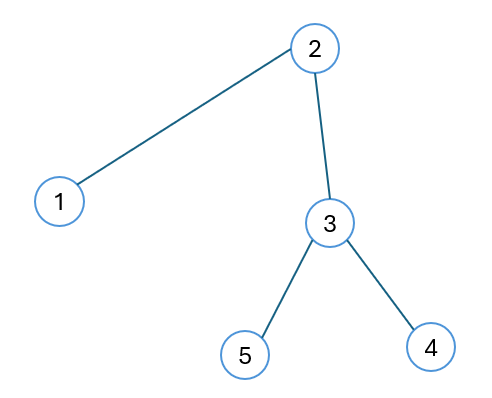
\includegraphics[scale=0.38]{img/undir_graph.PNG}
           \column{0.58\linewidth}
              $V = \{1,2,3,4,5\}$ \\
              $E = \{\{1,2\}, \{2,3\},\{3,4\},\{3,5\}\}$
         \end{columns} 

\end{frame}

\begin{frame}
\frametitle{Graph theory essentials}
Graph can be directed or undirected

\begin{columns}
  \column{0.38\linewidth}
     \centering
     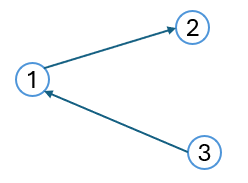
\includegraphics[scale=0.38]{img/dir_graph.PNG}
   \column{0.58\linewidth}
      $E = \{(1,2), (3,1)\}$
\end{columns} 

Graphs can be weighted, i.e. exists $W: E \to \mathbb{R}$

\begin{columns}
  \column{0.38\linewidth}
     \centering
     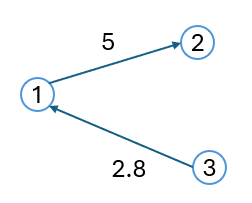
\includegraphics[scale=0.38]{img/weighted_graph.PNG}
   \column{0.58\linewidth}
      \begin{flalign*}
          &E = \{(1,2), (3,1)\} \\
          &W((1,2)) = 5 \\
          &W((3,1)) = 2.8 &&
      \end{flalign*}
\end{columns} 

\end{frame}

\begin{frame}
\frametitle{Graph theory essentials}
Graphs can be represented using adjacency matrix $\mathbb{A}$, whose entries are
\begin{equation}
    a_{ij} = \begin{cases}
1 \text{ if there is an edge $i \to j $}\\
0 \text{ otherwise}
\end{cases}
\end{equation}

Weighted graphs can be represented by weighted adjacency matrix $\mathbb{W}$, such that
\begin{equation}
    w_{ij} = \begin{cases}
\text{weight of an edge $i \to j$ if the edge is present}\\
0 \text{ otherwise}
\end{cases}
\end{equation}
\end{frame}

\subsection{Graph properties}
\begin{frame}
\frametitle{Graph properties}  

\begin{columns}
  \column{0.5\linewidth}
    Degrees: 
    \begin{itemize}
        \item Undirected: $k_i = \sum_{i=1}^{N} a_{ij}$
        \item Directed: \\ \hspace{10px} $k_i^{in} = \sum_{i=1}^{N} a_{ji}$ \\
        \hspace{10px} $k_i^{out} = \sum_{i=1}^{N} a_{ij}$
    \end{itemize}
   \column{0.5\linewidth}
     Strengths: 
    \begin{itemize}
        \item Undirected: $s_i = \sum_{i=1}^{N} w_{ij}$
        \item Directed: \\ 
        \hspace{10px}$s_i^{in} = \sum_{i=1}^{N} w_{ji}$ \\
        \hspace{10px}$s_i^{out} = \sum_{i=1}^{N} w_{ij}$
    \end{itemize}
\end{columns} 
\vspace{30px}
\centering
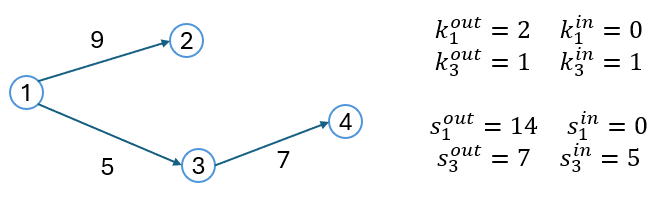
\includegraphics[scale=0.5]{img/degrees_strengths.png}
\end{frame}

\begin{frame}
\frametitle{Graph properties}  

\begin{columns}[t]
  \column{0.5\linewidth}
    Average nearest neighbor degree (ANND): 
    \begin{itemize}
        \item Undirected:  $k_{i}^{nn} = \frac{\sum_{j\neq i}a_{ij} k_j}{k_i}$
        \item Directed:
        \hspace{10px} $k_{i}^{nn,out} = \frac{\sum_{j\neq i}a_{ij} k_j^{out}}{k_i^{out}}$ \\
        \hspace{10px}$k_{i}^{nn,in} = \frac{\sum_{j\neq i}a_{ij} k_j^{in}}{k_i^{in}}$
    \end{itemize}
   \column{0.5\linewidth}
     Local clustering coefficient (undirected)
     $c_i = \frac{\sum_{j\neq i}\sum_{k\neq i,j}a_{ij} a_{jk} a_{ki}}{\sum_{j\neq i}\sum_{k\neq i,j}a_{ij}a_{ki}}$
\end{columns} 

\end{frame}

\subsection{Complex networks}
\begin{frame}
\frametitle{Complex networks}  
Complex networks
\begin{itemize}
    \item Do not have simple or regular structure - their topology is complex
    \item Are observed in many real-world situations:
    \begin{itemize}
        \item Citations network
        \item Protein-protein interactions
        \item World-wide web
        \item World trade network
        \item Many others...
    \end{itemize}
\end{itemize}

Complex networks theory tries to find models, which can replicate properties of real-world networks.

\end{frame}

\section{Random graph models}
\begin{frame}{Random graph models}
    In general, random graph models are such models, which to each graph $G$ from given set $\mathcal{G}$ assign a probability $P(G)$, \\ s.t. $\sum_{G \in \mathcal{G}}P(G) = 1$ \\
    \vspace{30px}
    We may call these methods \textit{ensemble models}, instead of generating single graph, we have a whole ensemble of graphs.
\end{frame}

\subsection{Exponential random graphs}

\begin{frame}{Exponential random graphs}
\begin{itemize}
    \item Approach analogical to statistical physics
    \item Prescribes to find such a probability, which maximizes the Shannon entropy
    \begin{equation*}
        S = -\sum_{G \in \mathcal{G}}P(G) \ln P(G)
    \end{equation*}
    \item Canonical ensemble is obtained by imposing soft constraints
    \begin{equation*}
    c_i^* = \sum_{G \in \mathcal{G}} c_i(G)P(G)
    \end{equation*}
\end{itemize}
\end{frame}

\begin{frame}{Exponential random graphs}
\begin{itemize}
    \item Constrained maximization leads to
    \begin{equation*}
    P(G|\vec{\theta}) = \frac{e^{-H(G,\vec{\theta})}}{Z(\vec{\theta})}
\end{equation*}
where $H(G,\vec{\theta}) = \sum_{i=1}^k c_i(G)\cdot\theta_i$ is the graph Hamiltonian and $Z(\vec{\theta}) = \sum_{G \in \mathcal{G}}e^{-H(G,\vec{\theta})}$ is the partition function.
\item For example, one can use degrees as constraints
    \begin{equation}
        H(G,\vec{\theta}) = \sum_{i\neq j}\theta_i k_i(G)
    \end{equation}
\end{itemize}
\end{frame}

\subsection{Scale-invariant model}
\begin{frame}{Scale-invariant model}
The goal is to find a model, which is consistent across multiple scales
\centering
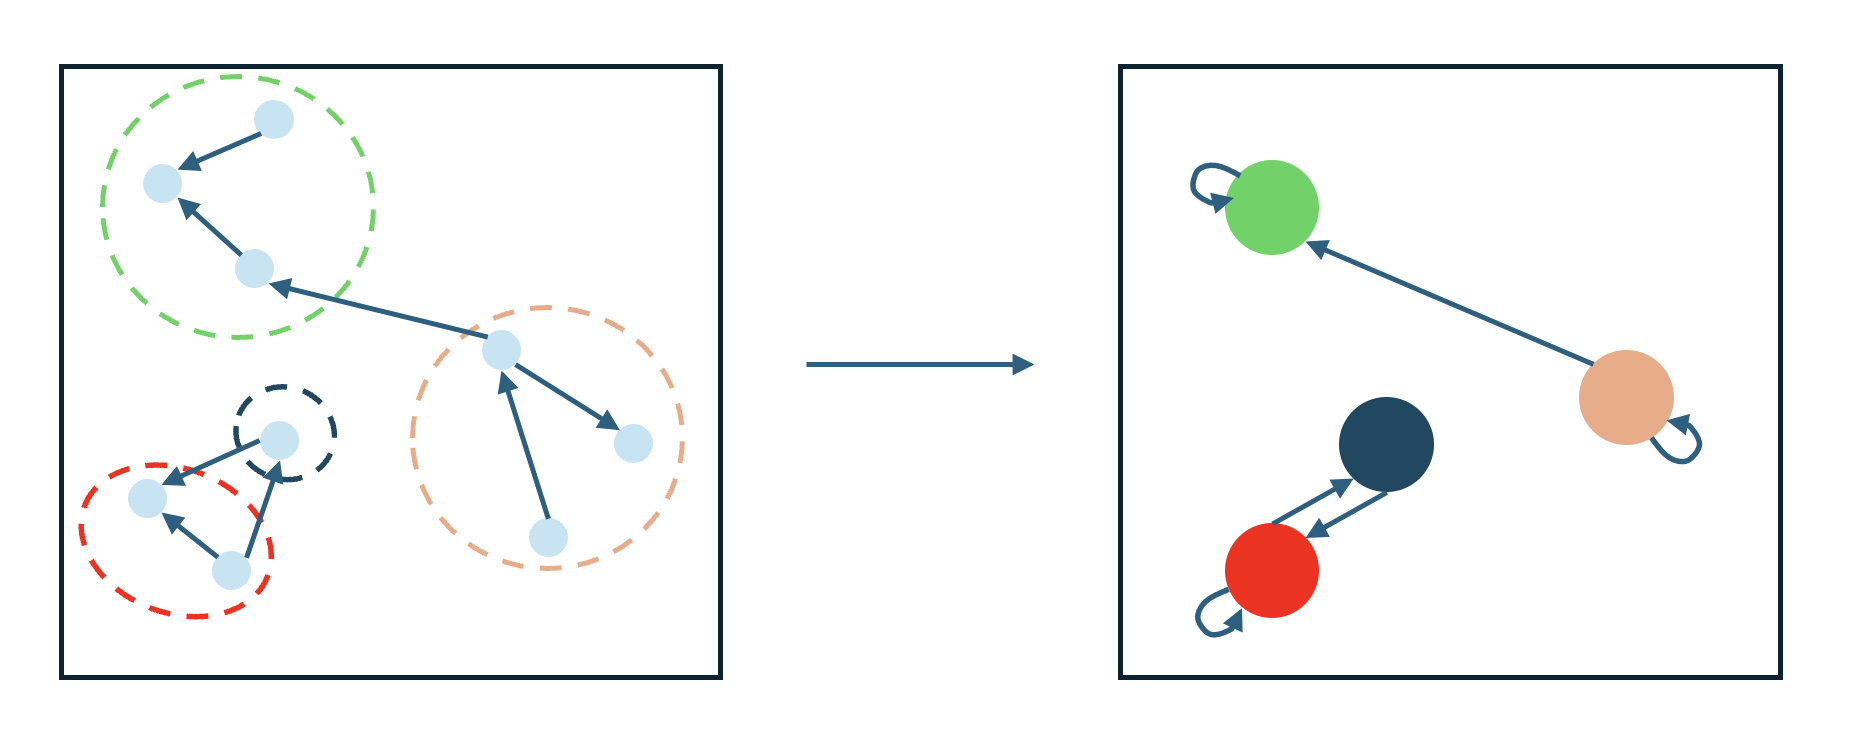
\includegraphics[scale=0.35]{img/coarse_graining.png}    
\end{frame}
\begin{frame}{Scale-invariant model}
    \begin{itemize}
        \item Assumes the following parameters
        \begin{itemize}
            \item each node $i$ has the so-called fitness $x_i$ determining its tendency to form connections
            \item $z$ for overall density
        \end{itemize}
        \item Also assumes, that upon coarse-graining, the fitnesses are additive, i.e. for a block-node $I$, its fitness $x_I = \sum_{i\in I} x_i$
        \item Lastly, it assumes that edges are independent random variables
        \item Having these assumptions, the aim is to find such a model, whose graph probability has the same form for all possible coarse-grainings and where only parameters change using some renormalization rule.
    \end{itemize}
\end{frame}

\begin{frame}{Scale-invariant model}
It was shown \footcite{Garuccio2023} that these assumptions lead to a link probability

\begin{equation*}
    p_{ij} = 1 - \exp(-zx_i x_j)
\end{equation*}

For directed case, one can assume existence of outward fitnesses $x_i$ and inward fitnesses $y_i$. Then one obtains a model

\begin{equation*}
    p_{ij} = 1 - \exp(-zx_i y_j)
\end{equation*}

The links are independent, therefore the random graph model is fully defined (probability of graph is product of link probabilities)
\end{frame}

\section{Network reconstruction}
\begin{frame}{Network reconstruction}
\begin{itemize}
    \item The goal is to plausibly reconstruct a given empirical network using only partial information about it
    \item For example, we want to find a reconstruction using only the knowledge of node out-strengths, in-strengths and number of links
    \item In such case, we want to find $O(N^2)$ entries of weighted adjacency matrix, using only the knowledge of $O(N)$ strengths.
    \item We may try to find one reconstructed network, however, the more robust approach is to generate an ensemble and then evaluating properties over the whole ensemble
    \item Example: interbank network
\end{itemize}
\end{frame}

\begin{frame}{Interbank network}
\begin{itemize}
    \item Interbank network is a network of loans between banks
    \item It is a weighted network, where each link corresponds to a loan and its weight is the amount of the loan
    \item Banks do not disclose their individual loans, they only announce their total assets and liabilities, i.e. for bank $i$, we know $A_i$ and $L_i$
    \item In terms of network properties, this corresponds to strengths $A_i = s_{0,i}^{in}$, $L_i = s_{0,i}^{out}$
    \item To study dynamical processes like stress-propagation, we need to know the full weighted adjacency matrix, therefore a reconstruction method is needed
\end{itemize}
\end{frame}

\begin{frame}{Max-Ent algorithm}
Prescribes to maximize
\begin{equation*}
    S = -\sum_{i,j=1}^N w_{ij}\ln w_{ij}
    \label{eq_max_ent_entropy}
\end{equation*}
Leads to
\begin{equation}
    w_{ij}^{ME} = \frac{s_{0,i}^{out}s_{0,j}^{in}}{\hat{W}} \qquad \forall i, j
\end{equation}
where $\hat{W} = \sum_{i=1}^N s_{0,i}^{out} = \sum_{i=1}^N s_{0,i}^{in}$.
However, if all strengths are nonzero, then all entries of the weighted adjacency matrix are nonzero - fully connected network
\end{frame}

\begin{frame}{Two step algorithms}
    We can divide the reconstruction in two steps
    \begin{enumerate}
        \item First, we use some method to find the the topology of the reconstructed network (i.e. we find the adjacency matrix)
        \item Only after that we assign weights
    \end{enumerate}
    Several successful methods like that were proposed. \footcite{Squartini2018}
\end{frame}

\section{NR using SIM}
\subsection{Using the original SIM}
\begin{frame}{Network reconstruction using the Scale-invariant model}
Motivation: the Scale-invariant model might work better than other methods in situations, where different scales are present simultaneously.\\
\vspace{30px}
For example, we know detailed information about banks in Czech republic, but only aggregate information about all banks in France, i.e. banks of France form only one node in our network.
\end{frame}
\begin{frame}{Network reconstruction using the Scale-invariant model}
We assume the knowledge of node out-strengths $x_i \equiv s_{0,i}^{out}$, in-strengths $y_i \equiv s_{0,i}^{in}$ and the total number of links $L_0$


We propose to use the following two step model
    \begin{enumerate}
        \item Sample edges using the connection probability given by the Scale-invariant model, i.e.
        \begin{equation*}
            p_{ij}^{SIM} = 1 - \exp(-zx_i y_j)
        \end{equation*}
        \item Assign weights using the corrected gravity model \begin{equation}
        w_{ij} = \begin{cases}
            0 \qquad &\text{if } a_{ij} = 0\\
            \frac{x_i y_j}{W p_{ij}^{SIM}} &\text{if } a_{ij} = 1
        \end{cases}    
    \end{equation}
    where $W \equiv \sum_{i=1}^N x_i =  \sum_{i=1}^N y_i$
    \end{enumerate}
\end{frame}

\begin{frame}{Network reconstruction using the Scale-invariant model}
Before sampling edges, we need to find the value of $z$. We do that by fitting the expected number of links over an ensemble to the empirical value
\begin{equation*}
        \langle L \rangle = \mathbb{E}(\sum_{i,j=1}^{N} a_{ij}) = \sum_{i,j=1}^{N} p_{ij} = \sum_{i,j=1}^{N} (1 - \exp(-z x_i y_j)) \overset{!}{=} L_0
    \end{equation*}

\end{frame}

\begin{frame}{Network reconstruction using the Scale-invariant model}
To evaluate our method, we might want to try reconstructing some real-world network. The primary aim is the interbank network, however, there is no dataset publicly available. \\
\vspace{30px}

In this research project, we used the network of flights between 1021 US cities in the year 2015. Weights are numbers of passengers. The total number of links in our network is 19199.

\end{frame}

\begin{frame}{Results}
    \begin{figure}[!ht]
    \centering
    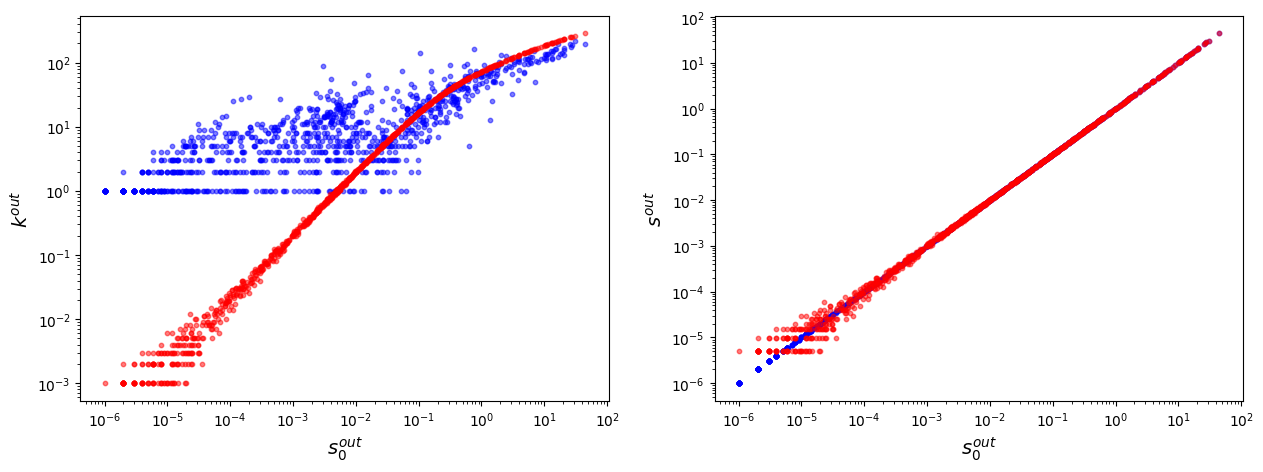
\includegraphics[scale=0.35]{img/Vanilla_SIM/deg_strengths_rec.png}
\end{figure}
\end{frame}

\begin{frame}{Results}
    \begin{figure}[!ht]
    \centering
    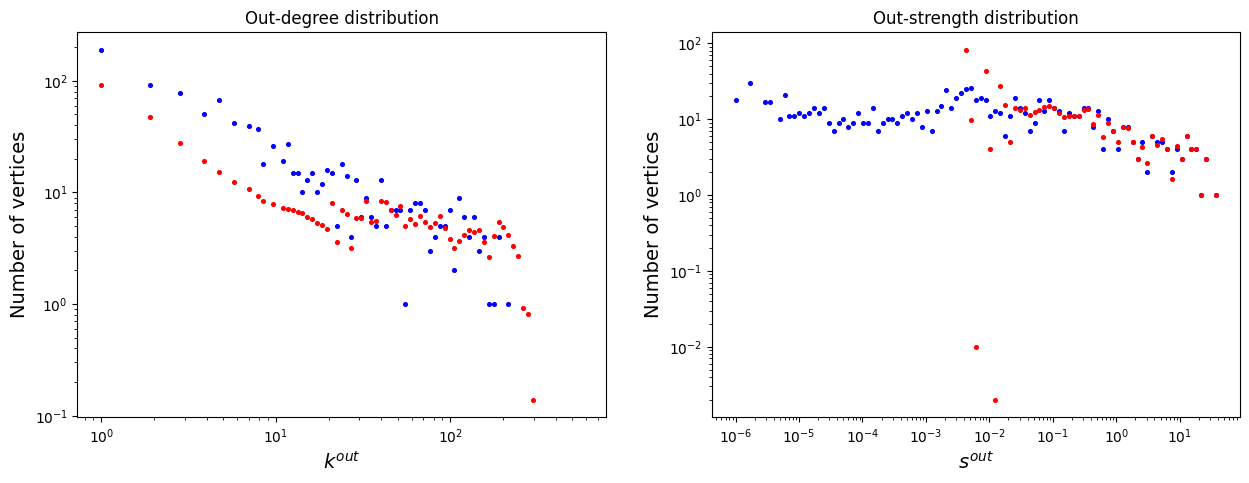
\includegraphics[scale=0.35]{img/Vanilla_SIM/deg_strengths_hist_rec.png}
\end{figure}
\end{frame}

\begin{frame}{Results}
    \begin{figure}[!ht]
    \centering
    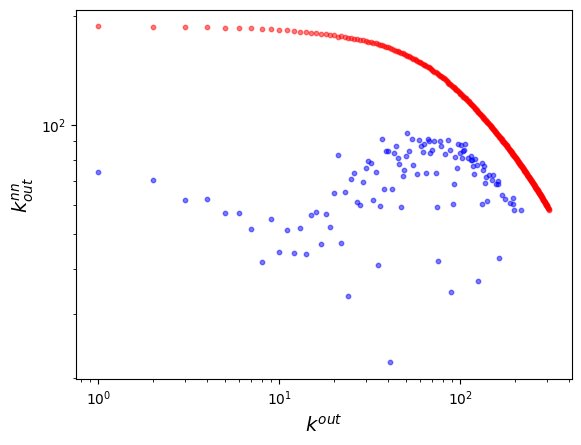
\includegraphics[scale=0.35]{img/Vanilla_SIM/ANND_k.png}
\end{figure}
\end{frame}

\begin{frame}{Results}
    \begin{figure}[!ht]
    \centering
    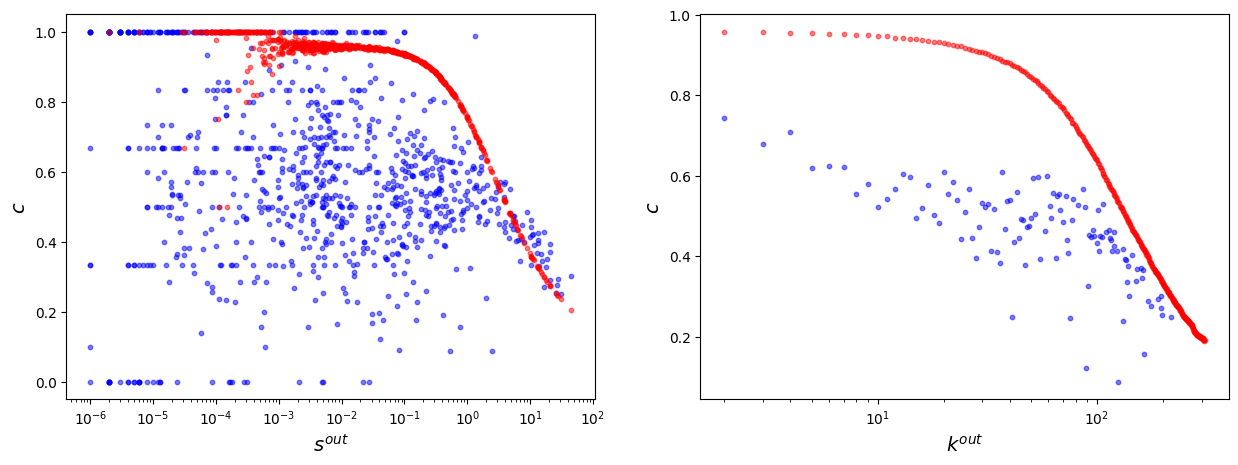
\includegraphics[scale=0.35]{img/Vanilla_SIM/cl_coeff.png}
\end{figure}
\end{frame}

\subsection{Out-degree corrected SIM}
\begin{frame}{Correction of degrees}
  We encountered a significant problem: too many isolated nodes
\begin{itemize}
    \item Out of 1021 nodes, there were on average 502.745 out-isolated nodes and 503.166 in-isolated nodes in the reconstructed ensemble
    \item However, all nodes in the empirical network have nonzero strength, therefore are not isolated
    \item This can lead to poor results when evaluating stress-propagation on the network
\end{itemize}  
\end{frame}

\begin{frame}{Out-degree corrected SIM}
  Let us first demand that all out-degrees must be nonzero. How to modify the original model in the most ``unbiased'' way?
  
  In such case, our space of allowed graphs is smaller, we denote it $\Gamma$. On this space, we can define
\small
  \begin{align*}
    P_{oDSIM}\left(\{a_{ij}\}_{i,j=1}^N\right) &= P_{SIM}\left(\{a_{ij}\}_{i,j=1}^N \,|\, k_i^{out} > 0 \, \forall i\right)\\ &=\frac{P_{SIM}\left(\{a_{ij}\}_{i,j=1}^N\right)}{P_{SIM}\left(k_i^{out} > 0 \, \forall i\right)} \qquad \forall \{a_{ij}\}_{i,j=1}^N \in \Gamma
\end{align*}
\normalsize
  
\end{frame}

\begin{frame}{*Analytical derivation}
  Since rows of the adjacency matrix remain independent, the denominator can be analytically computed
  \begin{equation*}
      P_{SIM}\left(k_i^{out} > 0 \, \forall i\right) = \prod_i P_{SIM}\left(k_i^{out} > 0\right)
  \end{equation*}
 and 
 \begin{align*}
    P_{SIM}(k_i^{out} > 0) &= 1-P(k_i^{out}=0) = 1 - \prod_j(1-p_{ij}) = \\ &=1 - \prod_j\exp(-zx_i y_j) 
    = 1 - \exp(-zx_i\sum_j y_j) = \\ &= 1 - \exp(-zx_i W)
\end{align*}
  
\end{frame}

\begin{frame}{Results}
    Although the number of out-isolated nodes decreased to zero, the number of in-isolated nodes stayed basically untouched
\end{frame}

\subsection{Degree corrected SIM}
\begin{frame}{Degree corrected SIM}
  What if we demand, that both out-degrees and in-degrees shall be nonzero?

  This once again defines a restricted space of graphs $\Gamma$, on which we can define the corretced model as

\footnotesize
  \begin{equation*}
    P_{DSIM}\left(\{a_{ij}\}_{i,j=1}^N\right) = \frac{P_{SIM}\left(\{a_{ij}\}_{i,j=1}^N\right)}{P_{SIM}\left((k_i^{out} > 0 \, \forall i) \cap (k_i^{in} > 0 \, \forall i )\right)} \qquad \forall \{a_{ij}\}_{i,j=1}^N \in \Gamma
\end{equation*}
  
\normalsize
  
\end{frame}

\begin{frame}{Degree corrected SIM}
Now, we made all entries of the adjacency matrix dependent. Computation of the denominator is rather involved. And even if we compute it, we would need to sample the whole graph at once.

\vspace{30px}
Instead, we propose to use the Metropolis-Hastings algorithm.
\end{frame}

\begin{frame}{Metropolis-Hastings algorithm - key features}
    \begin{itemize}
        \item Markov chain Monte Carlo algorithm for sampling from probability distributions
        \item Generates a sequence of samples, next sample is accepted or rejected based on ratio of probabilities
        \item That makes it possible to avoid the computation of the denominator
        \item At each step, we can flip one entry of the adjacency matrix, which makes the ratio of probabilities rather simple
    \end{itemize}
\end{frame}

\begin{frame}{Results}
\begin{figure}[!ht]
    \centering
    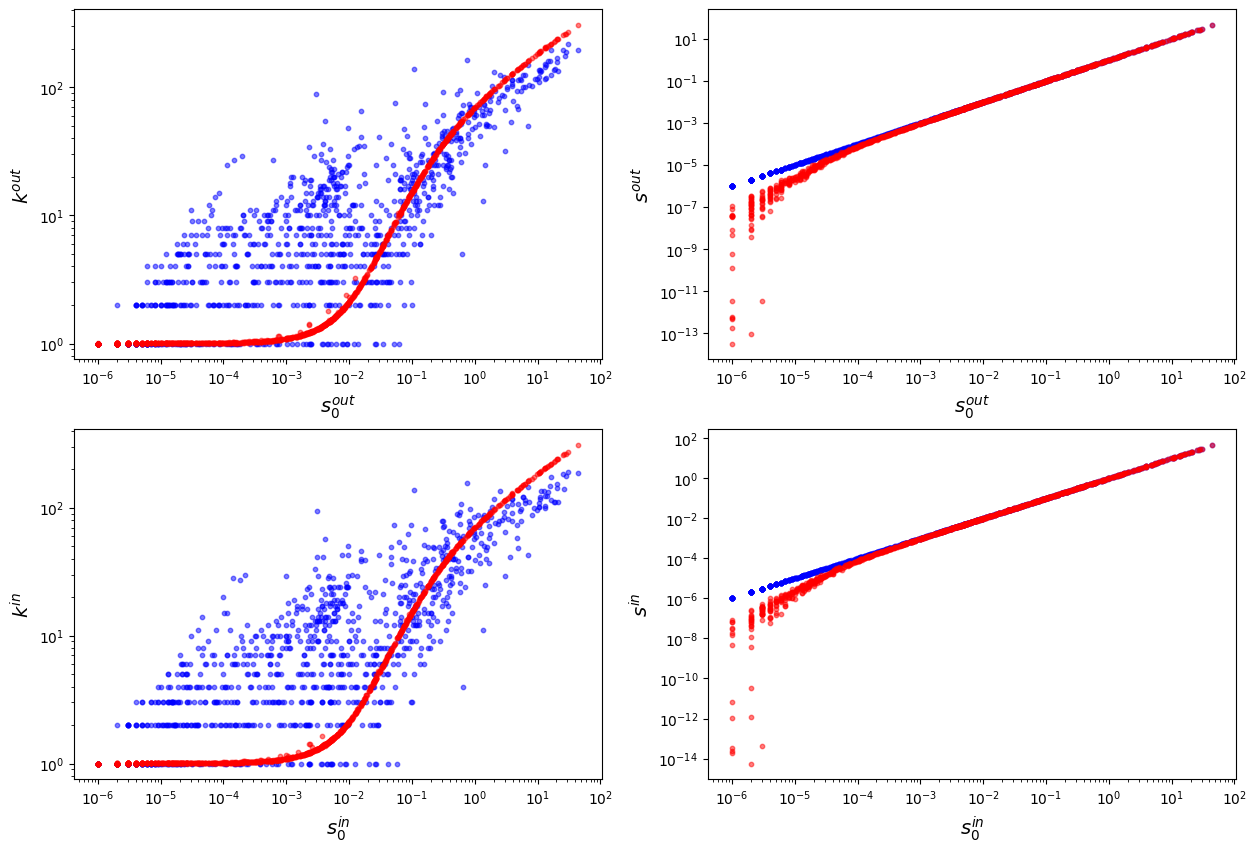
\includegraphics[scale=0.3]{img/Degree_corrected/degrees_strengths_rec.png}
\end{figure}
\end{frame}

\begin{frame}{Results}
\begin{figure}[!ht]
    \centering
    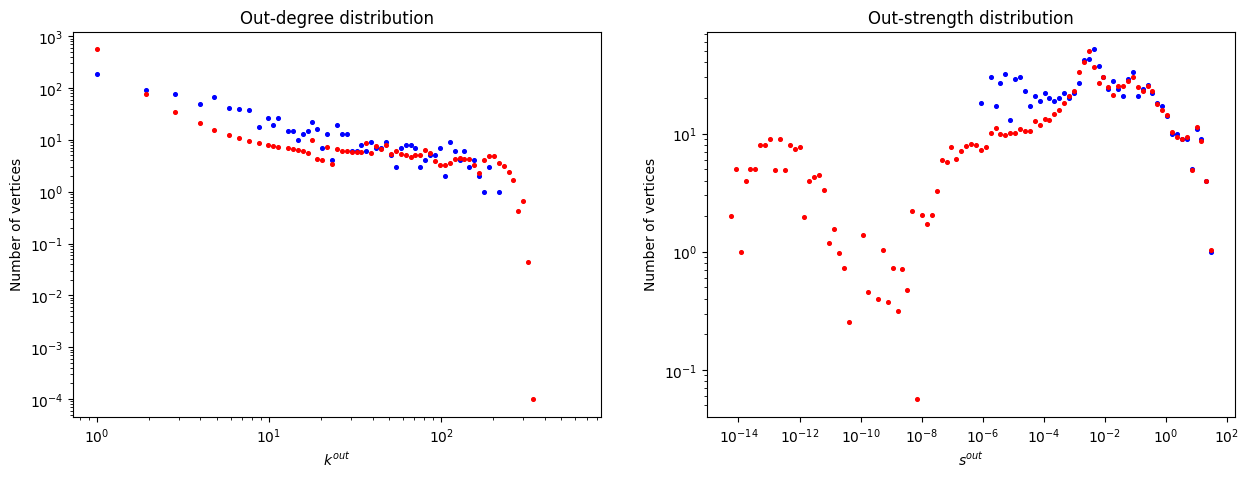
\includegraphics[scale=0.3]{img/Degree_corrected/degrees_strengths_hist.png}
\end{figure}
\end{frame}

\begin{frame}{Results}
\begin{figure}[!ht]
    \centering
    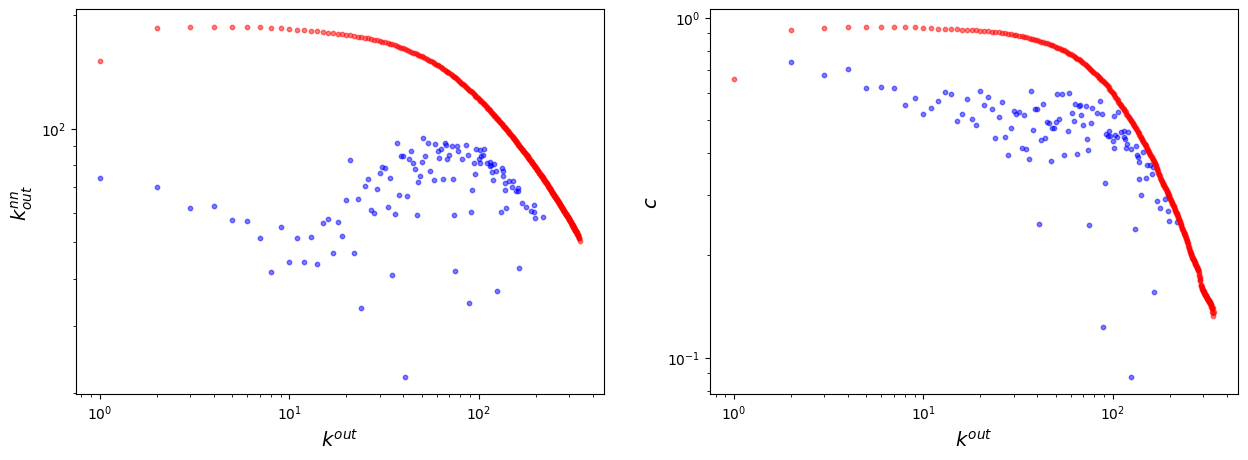
\includegraphics[scale=0.3]{img/Degree_corrected/annd_k_cl_coeff_k.png}
\end{figure}
\end{frame}

\begin{frame}{Results}
\begin{figure}[!ht]
    \centering
    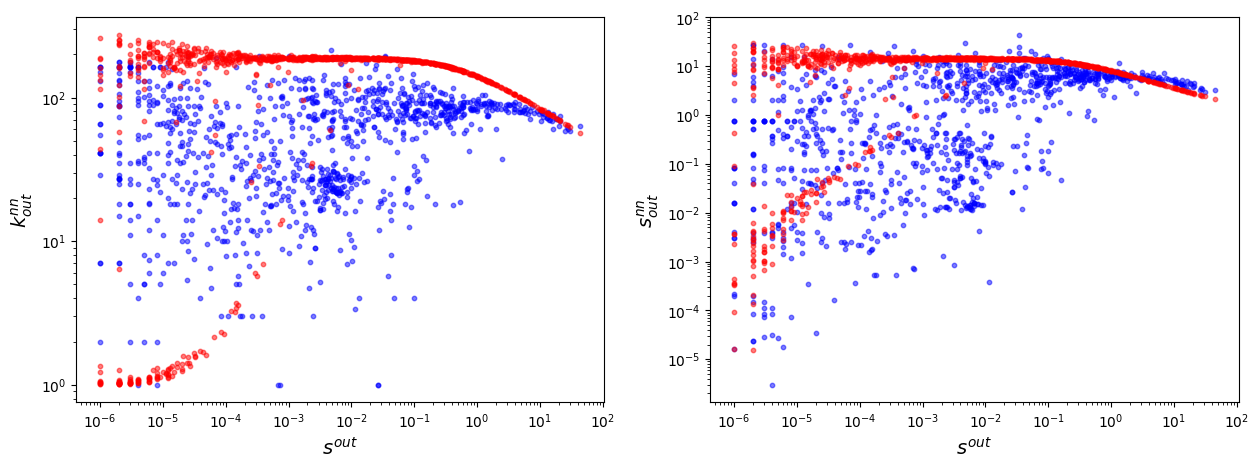
\includegraphics[scale=0.3]{img/Degree_corrected/annd_anns.png}
\end{figure}
\end{frame}

\begin{frame}{Results}
\begin{figure}[!ht]
    \centering
    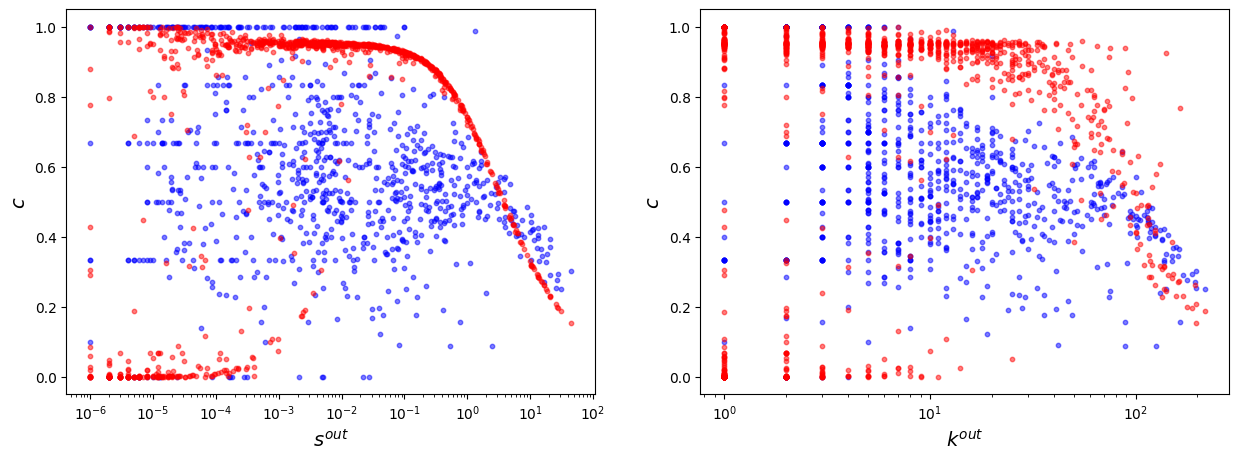
\includegraphics[scale=0.3]{img/Degree_corrected/cl_coeff.png}
\end{figure}
\end{frame}

\section*{Conclusion}
\begin{frame}{Conclusion}
Further work can be done 
\begin{itemize}
    \item Improving the sampling strategy
    \item Different models are applicable in different situations - test on the actual interbank network
    \item Comparison with already existing methods, showing possible advantage on multiscale data
    \item Study dynamical processes - stress propagation
\end{itemize}
\end{frame}

\printbibliography

\end{document}